\documentclass[10pt]{beamer}

\usepackage{enumitem}
\usepackage{graphicx}
\usepackage{amsmath,amssymb}
\usepackage{physics}
\usepackage{animate}
\usepackage[utf8]{inputenc}

\usetheme{Berlin}

\title[Optimisation and Backflow]{Wavefunction Optimisation and Backflow in Quantum Monte Carlo Simulations:}
\subtitle{}
\author[Clio Johnson]{Clio~Kennedy~Johnson}
%\institute[FST]{Faculty of Science and Technology}
\date[2023-10-17]{17th of October, 2023}
\titlegraphic{%
    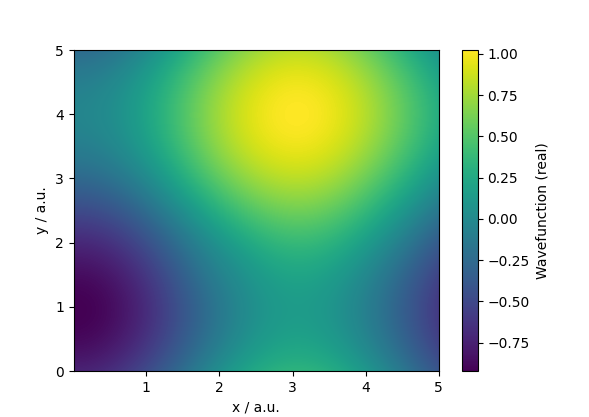
\includegraphics[scale=.29]{./images/heatmap2.png}
}

\begin{document}

\begin{frame}
    \titlepage%
\end{frame}


\begin{frame}
    \frametitle{Introduction \& Overview}
    \begin{itemize}
        \item[\textbullet] Introduction to quantum Monte Carlo (QMC) methods, particularly variational Monte Carlo (VMC).
        \item[\textbullet] A look at wavefunction types and optimisation
        \item[\textbullet] A brief exploration of backflow displacements
    \end{itemize}
\end{frame}


\begin{frame}[allowframebreaks]
    \frametitle{Quantum Monte Carlo (QMC)}
    \textbf{First of all, what is a Monte Carlo method?}\medskip\newline
    Monte Carlo are numerical methods that obtain a result through random sampling. They involve an overall picture generated from a large number ($\mathcal{N}$) of iterations.\medskip\newline
    They are useful for systems with many, \textit{many} degrees of freedom as the error in a result scales $\propto\frac{1}{\sqrt{N}}$ irrespective of the dimensionality of a system.\medskip\newline % Mention that this is a consequence of the Central Limit Theorem.
    You can do Monte Carlo integration on integrals that looks like this:
    \begin{equation}
        E = \int\dd{\vb{x}}\rho\pqty{\vb{x}}f\pqty{\vb{x}}
        \approx\sum_{n=1}^{\mathcal{N}}\frac{f\pqty{\vb{x}_n}}{\mathcal{N}}
    \end{equation}
    \framebreak%

    \textbf{A simple Monte Carlo Example:}\medskip\newline
    Compute $\pi$ from evaluating a circular integral:
    \begin{figure}
        \centering
        % Put a graphic of quarter circle MC integration here
        \animategraphics[controls,scale=0.25]{3}{./figs/pi_gif/pi_30K-}{0}{9}
        \caption{%
            By nicoguaro - Own work, CC BY 3.0,
            \url{https://commons.wikimedia.org/w/index.php?curid=14609430}
        }
    \end{figure}
    \framebreak%

    \textbf{What are QMC methods?}\medskip\newline
    QMC methods aim to solve many-body Schr\"odinger equations iteratively. They are used to estimate ground state energies of these many-body systems as well as optimise wavefunctions.\medskip\newline
    \begin{equation}
        \hat{H}=\sum\limits_{i}^{N_e}\frac{\nabla_i^2}{2}+\sum\limits_{i}^{N_e}\sum\limits_{j\neq i}^{N_e}\frac{1}{\vqty{\va{r}_{ij}}}-\sum\limits_{i}^{N_e}\sum\limits_{a}^{N_I}\frac{Z_a}{\vqty{\va{r}_{ia}}}+\sum\limits_a^{N_I}\sum\limits_b^{N_I}V_{ab}
    \end{equation}
    \framebreak%

    \textbf{Types of QMC}\medskip\newline
    There are two QMC algorithms that are most commonly used:
    \begin{itemize}
        \item[\textbullet] \textbf{Variational quantum Monte Carlo (VMC)}\newline
        Takes a trial wavefunction with electron positions, proposes a move in configuration space and then either accepts or rejects it according to the Metropolis-Hastings method.\newline
%       Other free parameters in the wavefunction can be optimised throughout the simulation. The simulation produces a variational estimate of the ground state energy through a rolling mean of local energies calculated at each iteration. The accuracy of this energy is dependent on a number of factors, including how well optimised the wavefunction parameters are.\newline
        \item[\textbullet] \textbf{Diffusion quantum Monte Carlo (DMC)}\newline
        DMC solves an imaginary time Schr\"odinger equation. A large number of configurations are diffused throughout the simulation, and their density is used to recover the ground state wavefunction. Most DMC simulations are \textbf{Fixed Node} DMC
    \end{itemize}
    \framebreak%

    \textbf{VMC Formulation}\medskip\newline
    Given a configuration of $N$ electrons denoted
    $\vb{R}=\pqty{\vb{r}_1,\vb{r}_2,\ldots,\vb{r}_N}$, with an $N$
    body Hamiltonian $\hat{H}$.\newline
    If we provide an approximate trial wavefunction $\psi_T\pqty{\vb{R}}$. The
    variational principle ensures:
    \begin{equation}
        \int\dd{\vb{R}}\psi_T^*\pqty{\vb{R}}\hat{H}\psi_T\pqty{\vb{R}}\geq E_0
    \end{equation}
    So we're free to see the configuration $\vb{R}$ as a set of variational
    parameters, used to optimise our trial wavefunction.
    \framebreak

    \textbf{VMC Formulation Continued}\medskip\newline
    A Markov chain Monte Carlo method called the Metropolis algorithm is used
    to sample a series of points from the probability density function
    $\vqty{\psi_T\pqty{\vb{R}}}^2$.\medskip\newline
    \begin{equation}
        \int\dd{\vb{R}}
        \vqty{\psi_T\pqty{\vb{R}}}^2
        E_L\pqty{\vb{R}}
        \geq E_0,
    \end{equation}
    where
    \begin{equation}
        E_L\pqty{\vb{R}}=\frac{\hat{H}\psi_T\pqty{\vb{R}}}{\psi_T\pqty{\vb{R}}}.
    \end{equation}
    \framebreak

    \begin{figure}
        \centering
        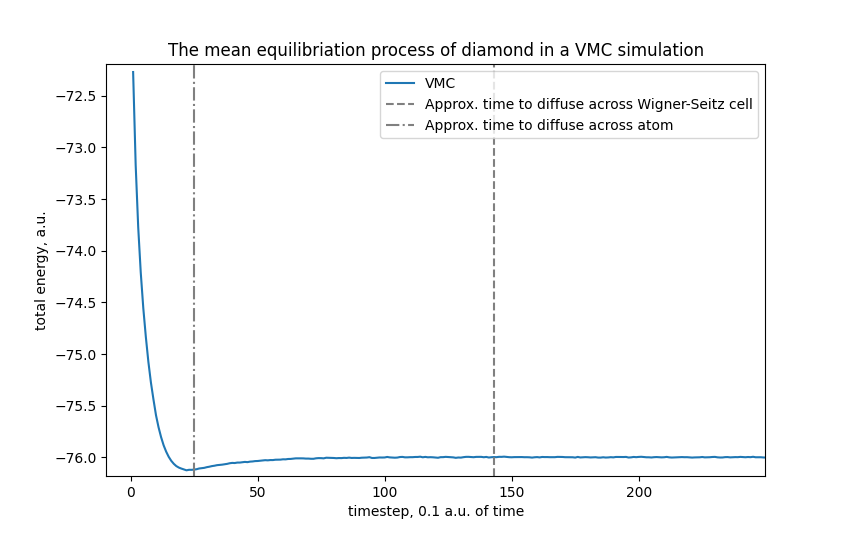
\includegraphics[scale=0.37]{./images/control_process_diamond_ae2.png}
        \caption{Recovered autocorrelation function from the mean of 40,000
        VMC simulations on 8 cell all-electron diamond.}
    \end{figure}
    \framebreak

    \begin{itemize}
        \item[\textbullet] \textbf{Diffusion quantum Monte Carlo (DMC)}\newline
        DMC propagates walkers through imaginary time, using a birth-death
        algorithm dictated by the trial wavefunction $\psi_T$, and evaluating
        the ground state energy based on regions of walker density.
        \item Note! It relies on the fixed node approximation.
    \end{itemize}
    \framebreak

    \textbf{Fixed Nodes!}
    \begin{itemize}
        \item[\textbullet] DMC uses regions of positive walker density.
        \item[\textbullet] Nodes are points at which $\psi_T\pqty{\vb{R}}=0$.
        \item[\textbullet] Remember our system is $3N$ Dimensional.
        \item[\textbullet] Nodal structure of the wavefunction is a $3N-1$
        dimensional hypersurface.
    \end{itemize}
    \framebreak

    \begin{figure}
        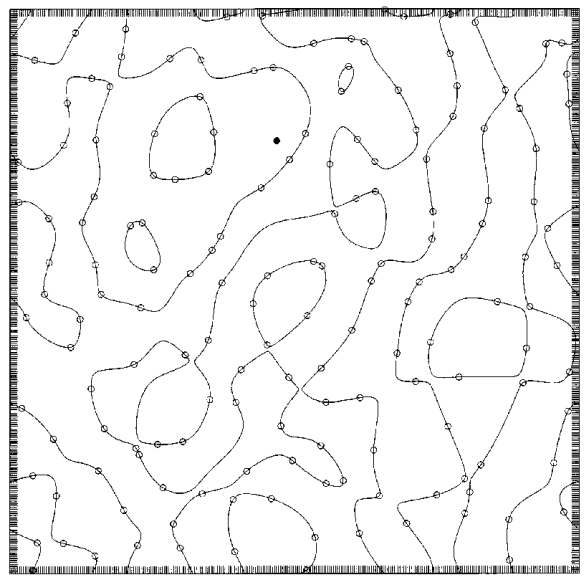
\includegraphics[scale=0.22]{./images/nodal-surface-slice.png}
        \caption{
            A "slice" of the nodal surface of a 161 electron wavefunction,
            courtesy of Foulkes \textit{et al.}\cite{Foulkes2001} and Ceperley \textit{et al.}.
        }
    \end{figure}
    \framebreak

    \begin{itemize}
        \item[\textbullet] We sometimes need to alter the nodal surface of our
        trial wavefunction!
        \item[\textbullet] This can be done through VMC wavefunction
            optimisation by implementing \textbf{backflow}.
    \end{itemize}

\end{frame}

\begin{frame}[allowframebreaks]
    \frametitle{Slater-Jastrow-backflow Wavefunctions}
    \begin{equation}
        \psi_T\pqty{\vb{R}}=\mathcal{D}\pqty{\vb{R}}\exp\pqty{J\pqty{\vb{R}}}
    \end{equation}
    Normally a trial wavefunction is of the Slater-Jastrow form.\newline
    $\mathcal{D}\pqty{\vb{R}}$ is a Slater determinant.\newline
    $J\pqty{\vb{R}}$ is a Jastrow factor.\newline
    \framebreak

    \textbf{Backflow Displacement}
    \begin{itemize}
        \item[\textbullet] Nodal surface is determined by
        $\mathcal{D}\pqty{\vb{R}}$.
        \item[\textbullet] We can simulate interaction by replacing $\vb{R}$
        with a bunch of pseudo-coordinates:
        \begin{equation}
            \vb{X}\pqty{\vb{R}}=\vb{R}+\vb{\xi}\pqty{\vb{R}}
        \end{equation}
        \item[\textbullet] We give $\vb{\xi}\pqty{\vb{R}}$ an appropriate form
        dependent on several variational parameters. Allowing us to optimise the
        nodal surface variationally\cite{LopezRios2006}.
        \item[\textbullet] Leading to a wavefunction of the following form:
        \begin{equation}
            \psi_T=\mathcal{D}\pqty{\vb{X}\pqty{\vb{R}}}\exp\pqty{J\pqty{R}}
        \end{equation}
    \end{itemize}
    \framebreak

    \textbf{How to calculate Backflow displacement}
    \begin{itemize}
        \item[\textbullet] Our approximation is comprised of two-body,
        electron-nucleus, and electron-electron-nucleus terms.
        \item[\textbullet] I am currently attempting to implement a three-body
        backflow contribution (electron-electron-electron interactions).
    \end{itemize}
    \framebreak

    \begin{align}
        \vb{\xi}_i\pqty{\vb{R}}=&
        \vb{\xi}_i^{\text{e-e}}\pqty{\vb{R}}+
        \vb{\xi}_i^{\text{e-n}}\pqty{\vb{R}}+
        \vb{\xi}_i^{\text{e-e-n}}\pqty{\vb{R}}+
        \vb{\xi}_i^{\text{e-e-e}}\pqty{\vb{R}}
        \\
        \vb{\xi}_i^{\text{e-e-e}}\pqty{\vb{R}}=&
        \sum\limits_{\substack{j\neq i\\j=1}}^{N}
        \sum\limits_{\substack{k\neq i\\k>j\\k=1}}^{N}
        \omega_A\pqty{r_{j'k'},r_{i'k'},r_{i'j'}}
        \pqty{\vb{r}_{ik'}\delta_{ij'}+\vb{r}_{ij'}\delta_{ik'}}+\nonumber\\
        &\omega_B\pqty{r_{j'k'},r_{i'k'},r_{i'j'}}
        \pqty{\vb{r}_{ik'}\delta_{ij'}+\vb{r}_{ij'}\delta_{ik'}}+\nonumber\\
        &\omega_C\pqty{r_{j'k'},r_{i'k'},r_{i'j'}}
        \pqty{\vb{r}_{ik'}\delta_{ij'}+\vb{r}_{ij'}\delta_{ik'}}
    \end{align}
    \framebreak

    \textbf{Truncated Polynomial form of $\omega$}
    \begin{gather}
        \begin{align}
            \omega\pqty{r_{j'k'},r_{i'k'},r_{i'j'}}=&
            \sum\limits_{l=0}^{N_\omega}
            \sum\limits_{m=0}^{N_\omega}
            \sum\limits_{n=0}^{N_\omega}
            c_{lmn}r_{j'k'}^lr_{i'k'}^mr_{i'j'}^n\nonumber\\
            &\times\pqty{L_\omega-r_{j'k'}}^C
            \Theta\pqty{L_\omega-r_{j'k'}}\nonumber\\
            &\times\pqty{L_\omega-r_{i'k'}}^C
            \Theta\pqty{L_\omega-r_{i'k'}}\nonumber\\
            &\times\pqty{L_\omega-r_{i'j'}}^C
            \Theta\pqty{L_\omega-r_{i'j'}}
        \end{align}\\
        \\
        \nonumber
        \text{Our variational parameters are:}\quad
        c_{lmnA},c_{lmnB},c_{lmnC},L_\omega
    \end{gather}
\end{frame}

\begin{frame}[allowframebreaks]
    \frametitle{No-Cusp Conditions}
    \textbf{Remember the Local Energy:}
    \begin{equation}
        E_L\pqty{\vb{X}\pqty{\vb{R}}}=\frac{
            \hat{H}\psi_T\pqty{\vb{X}\pqty{\vb{R}}}
        }{
            \psi_T\pqty{\vb{X}\pqty{\vb{R}}}
        }
    \end{equation}
    This will always contain a kinetic energy term:
    \begin{equation}
        \frac{
            \laplacian\psi_T\pqty{\vb{X}\pqty{\vb{R}}}
        }{
            \psi_T\pqty{\vb{X}\pqty{\vb{R}}}
        }
    \end{equation}
    Which we always want to be defined \textit{i.e.} $\psi_T$ must be twice
    differentiable. We demand this is also the case for the Slater determinant
    incorporating the backflow transformation.
    \framebreak

    Consider taking our configuration of $N$ electrons, and fixing the
    coordinates of all but two of them. We now have a problem which can be
    expressed in terms of a centre of mass and separation coordinate system:
    \begin{equation*}
        \pqty{\bar{\vb{r}}_{ij},\vb{r}_{ij}}
    \end{equation*}
    Our question becomes: What constraints ought to apply to
    $\vb{X}\pqty{\vb{R}}$ at the coalescence point such that the local energy,
    $E_L$, doesn't diverge.
    \framebreak

    Skipping over the worst parts of the derivation for now:\newline
    Recalling the kinetic contribution to local energy, we want to consider
    the limit as $r_{ij}$ goes to $0$:
    \begin{equation}
        \lim\limits_{r_{ij}\to 0}\frac{
            \laplacian\psi_T\pqty{\vb{X}\pqty{\vb{r}_{ij}}}
        }{
            \psi_T\pqty{\vb{X}\pqty{\vb{r}_{ij}}}
        }
    \end{equation}
    If the two electrons are indistinguishable (spin aligned), then the
    denominator must equal zero in the limit.\medskip\newline
    So to prevent problems at like-spin electron coalescence we demand
    \begin{equation}
        \lim\limits_{r_{ij}\to 0}\laplacian\psi_T\pqty{\vb{X}\pqty{\vb{R}}}=0
    \end{equation}
    \framebreak

    This is what allows us to derive conditions on the $c_{lmn}$ variational
    parameters. These are still in development, we've reached the limit of my
    research so far.\medskip\newline
    Here be dragons...
\end{frame}


\begin{frame}[allowframebreaks]
    \frametitle{Further Reading}
    \bibliographystyle{vancouver}
    \bibliography{refs}

\end{frame}

\end{document}
